\chapter{Réalisation et mise en oeuvre}
Ce chapitre aborde la mise en oeuvre et la réalisation, en présentant les outils de réalisation ainsi que le travail réalisé.
\newpage
\section{Outils de développement}
\subsection{Langages de programmation et développement}
\subsubsection*{Python}
Python est un langage de programmation objet, multi-paradigme et multiplate-forme.
Il favorise la programmation impérative structurée, fonctionnelle et orientée objet.
C'est un outil essentiel pour notre projet puisque nous avons utilisé Django.\\

\begin{figure}[h]
      \centering
        
\includegraphics[width=7cm,height=5cm]{img/python.jpg}
        \caption{Logo de Python}
\end{figure}
\subsubsection*{JavaScript}
JavaScript est un langage de  programmation qui nous permet d'implémenter des éléments complexes sur des pages Web. Chaque fois, une page Web ne se contente pas de rester là et affiche des informations statiques que nous pouvons consulter: affichage de mises à jour de contenu actualisées, de cartes interactives, de graphiques 2D et animés. Graphiques 3D, défilement de jukebox vidéo, etc.\\
Nous avons utilisé Java Script pour l'animation de quelque bouttons, et la coloration dynamique de quelques interfaces graphiques dans l'application.
\begin{figure}[h]
      \centering
        
\includegraphics[width=7cm,height=5cm]{img/javascript.png}
        \caption{Logo de JavaScript}
\end{figure}

\subsubsection*{HTML/CSS}
HTML, HyperText Markup Language, donne la structure et la signification du contenu en définissant ce contenu comme, par exemple, des en-têtes, des paragraphes ou des images.\\
CSS, or Cascading Style Sheets, est un langage de présentation créé pour styliser l'apparence du contenu, à l'aide, par exemple, de polices ou de couleurs.\\
\begin{figure}[h]
      \centering
        
\includegraphics[width=7cm,height=5cm]{img/HTMLCSS.png}
        \caption{Logo de HTML et CSS}
\end{figure}

\newline
\subsection{Environement de développement}
\subsubsection*{Django}
Django est un framework Web Python de haut niveau qui encourage un développement rapide et une conception propre et pragmatique. Conçu par des développeurs expérimentés, il prend en charge une grande partie des tracas du développement Web, il nous a permet  donc de nous concentrer sur l'écriture de notre application sans avoir à réinventer la roue. C'est gratuit, open source, sécurisé et rapide.\\
C'est l'outil le plus important pour la réalisation de ce projet, les développeurs originaux l'ont choisi pour sa bonne performance, et donc nous avons choisi de garder le même outil pour faciliter la tâche.
\begin{figure}[H]
      \centering
        
\includegraphics[width=7cm,height=4cm]{img/django-logo.jpg}
        \caption{Logo de Django}
\end{figure}
\newline

\subsubsection*{Visual Studio Code}
Visual Studio Code est un éditeur de code extensible développé par Microsoft pour Windows, Linux et macOS. Il est  open source et gratuit, supportant plusieurs langages.
\begin{figure}[H]
      \centering
        
\includegraphics[width=7cm,height=6cm]{img/VS.png}
        \caption{Logo de Visual Studio Code}
\end{figure}
\newline
\subsubsection{Docker}
Docker est un ensemble de produits en tant que service de plate-forme qui utilisent la virtualisation au niveau du système d'exploitation pour fournir des logiciels dans des packages appelés conteneurs. Les conteneurs sont isolés les uns des autres et regroupent leurs propres logiciels, bibliothèques et fichiers de configuration; ils peuvent communiquer entre eux par des canaux bien définis.
\begin{figure}[H]
      \centering
        
\includegraphics[width=7cm,height=6cm]{img/Docker_logo.jpeg}
        \caption{Logo de Docker}
\end{figure}

\\
\\
\\
\subsubsection*{PostgreSQL}
PostgreSQL, également connu sous le nom de Postgres, est un système de gestion de base de données relationnelle gratuit et open source qui met l'accent sur l'extensibilité et la conformité aux normes techniques. Il est conçu pour gérer une gamme de charges de travail, des machines uniques au Data Warehouse ou aux services Web avec de nombreux utilisateurs simultanés.\\
Il est utilisé dans ce projet pour la gestion des bases de données.
\begin{figure}[H]
      \centering
        
\includegraphics[width=7cm,height=4cm]{img/PostgreSQL.png}
        \caption{Logo de PostgreSQL}
\end{figure}

\newpage
\section{Réalisation}
\subsection*{S'authentifier:}
Chaque utilisateur a un username qui est simplement l'abréviation de son nom, et un mot de passe, mais le mode passe est le même :"passe", pour le chef de fillière il peut entrer avec le username "root". les interfaces affichées et leurs  droits d'accès dépendent évidement de la classe de l'utilisateur. 
\begin{figure}[H]
      \centering
        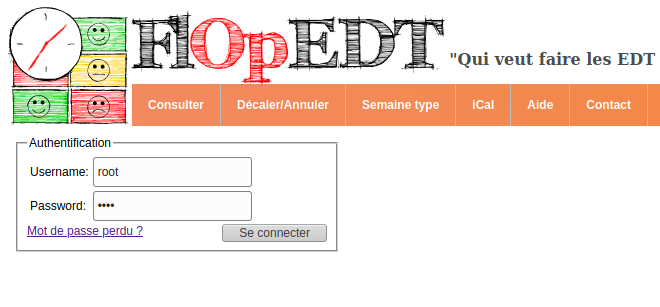
\includegraphics[width=14cm,height=12cm]{img/1.png}
        \caption{Interface login}
\end{figure}
\newpage
\subsection*{Semaine type:}
Si l'utilisateur est un prof, il peut accèder à l'interface "semaine type", pour séléctionner ses préférences, en d'autres termes les heures de son disponibilé et les heures de son non-disponibilité. \\
Il peut également chosir pour combien de semaine il veut garder cette semaine type.
\begin{figure}[H]
      \centering
        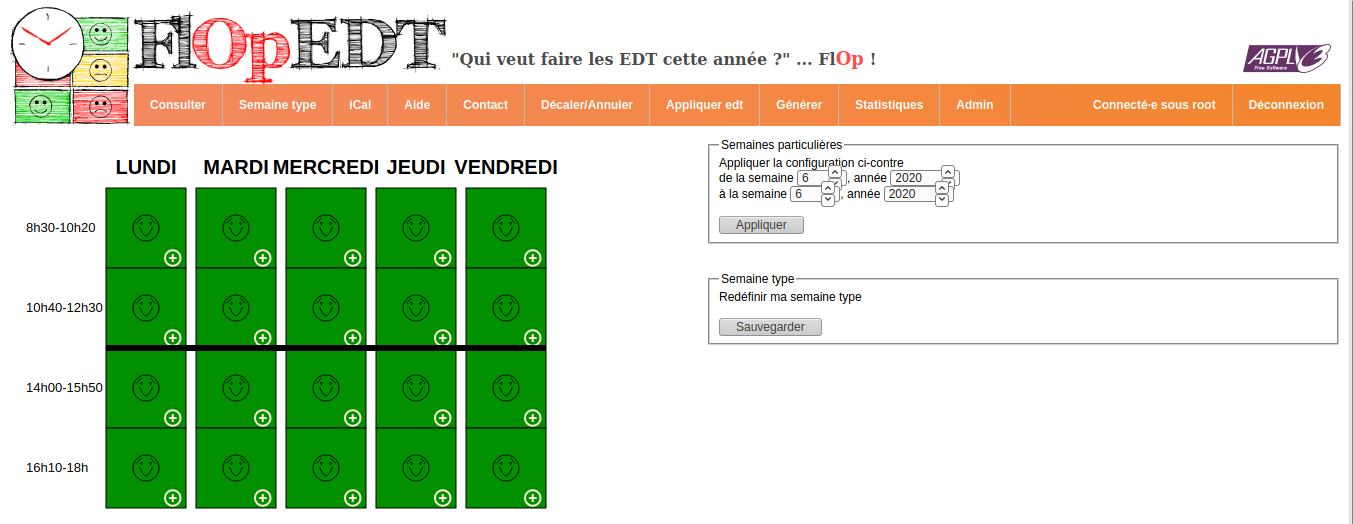
\includegraphics[width=14cm,height=12cm]{img/2.png}
        \caption{Interface Semaine type}
\end{figure}
\newpage
\subsection*{Emplois vide}
Lorsque l'utilisateur n'est pas encore connecté ou l'emplois est vide, cette interface va être affichée.
\begin{figure}[H]
      \centering
        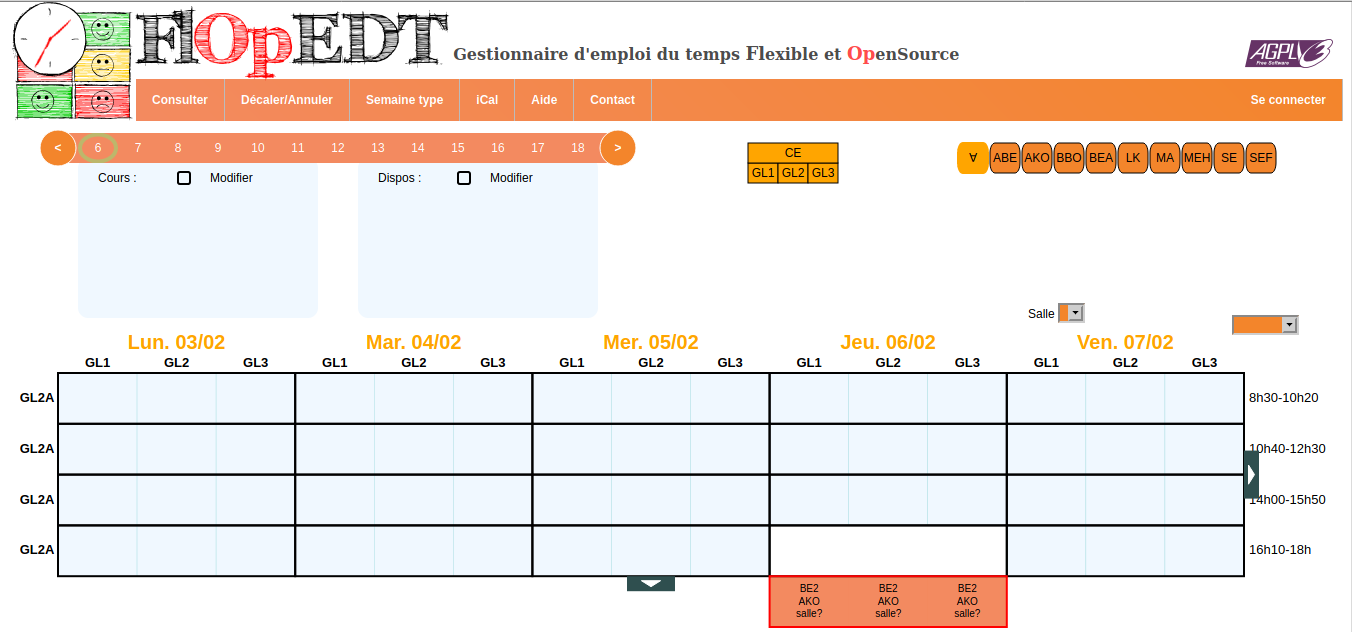
\includegraphics[width=15cm,height=12cm]{img/3.png}
        \caption{Interface Emplois vide}
\end{figure}
\newpage
\subsection*{Générer un Emplois:}
Le chef de fillière a le droit de générer l'emplois du temps via cette interface.
\begin{figure}[H]
      \centering
        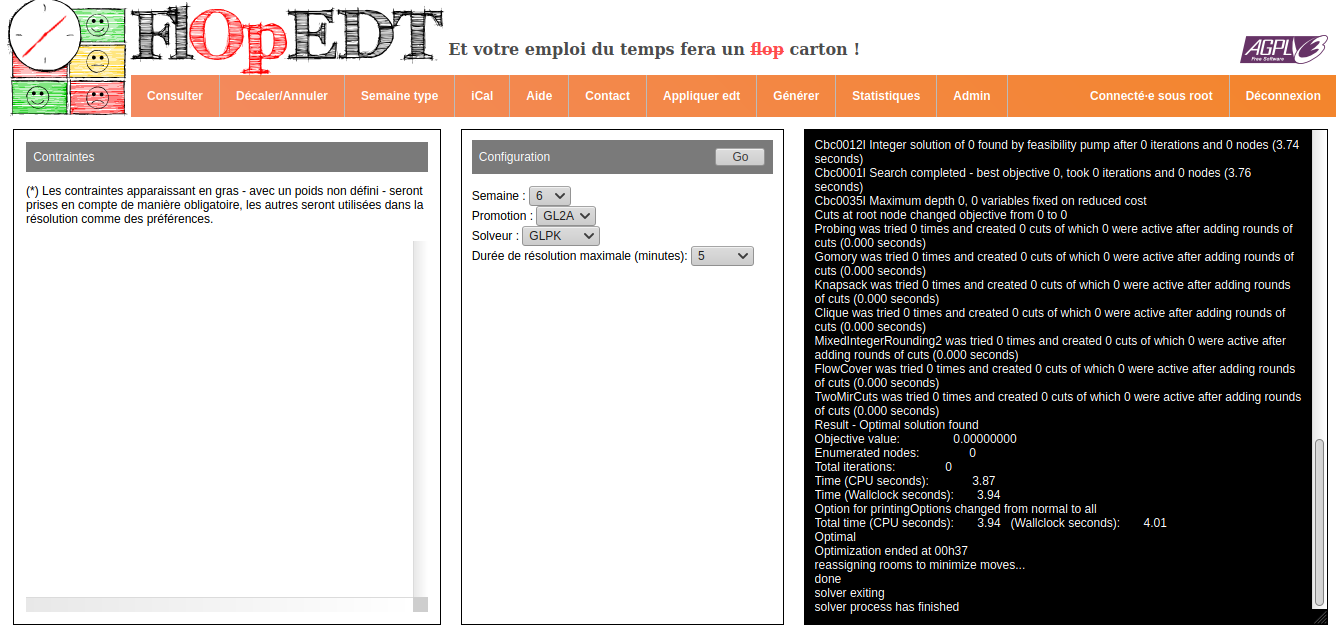
\includegraphics[width=15cm,height=12cm]{img/4.png}
        \caption{Interface générer emplois du temps}
\end{figure}
\newpage

\subsection*{Emplois générée}
Voilà notre emplois du temps, ce dernier peut étre modifié que par le chef de fillière via l'option modifier.
\begin{figure}[H]
      \centering
        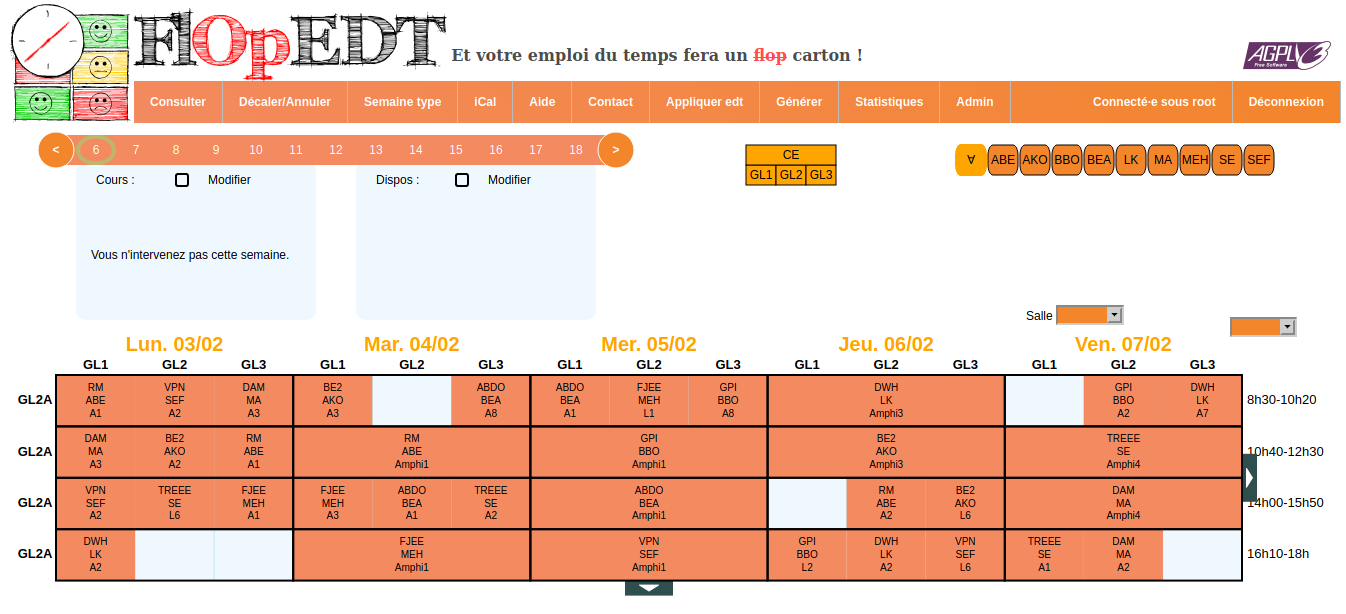
\includegraphics[width=15cm,height=12cm]{img/5.png}
        \caption{Interface Emplois généré}
\end{figure}
\newpage
\subsection*{Sauvegarder emplois du temps}
Si le chef de fillière est satisfait du résultat qu'il a eu, il peut sauvegarder l'emplois du temps pour toute la période.
\begin{figure}[H]
      \centering
        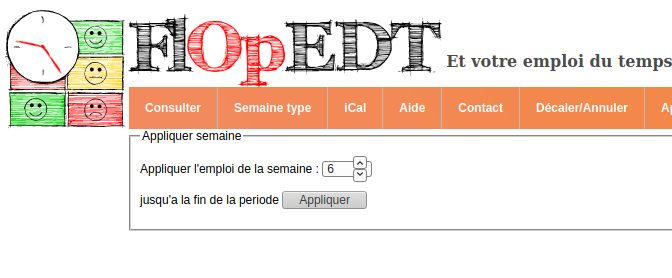
\includegraphics[width=15cm,height=12cm]{img/6.png}
        \caption{Sauvegarder emplois du temps}
\end{figure}
\newpage

\subsection*{Repporter ou annuler un cours}
Si le prof pour une raison quelconque veut repporter ou même annuler un cours, il peut le faire via cette interface, il doit d'abord préciser quel cours et avec quel groupe, et quand il va étre rattrappé.
\begin{figure}[H]
      \centering
        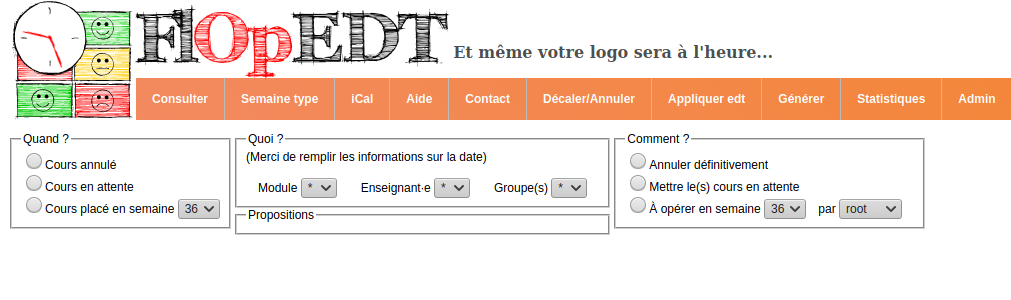
\includegraphics[width=15cm,height=12cm]{img/7.png}
        \caption{Interface repporter et annuler un cours}
\end{figure}
\newpage










